\section{Общие принципы автоматизации образовательной деятельности с помощью ostis-систем}
\label{sec_general_principles_automation_educational_activities}

\begin{SCn}
	
	\bigskip
	
	\begin{scnrelfromlist}{ключевое понятие}
		\scnitem{интеллектуальная обучающая система}
		\scnitem{семантический электронный учебник}
		\scnitem{компьютерные средства обучения}
		\scnitem{обучение пользователя компьютерной системы}
	\end{scnrelfromlist}
	
	\bigskip
	
	\begin{scnrelfromlist}{ключевое знание}
		\scnitem{Этапы преобразования традиционного учебника в семантический электронный учебник}
		\scnitem{Предметная область методов и средств реализации целенаправленного и персонифицированного процесса обучения пользователей для каждой ostis-системы, входящей в состав \textit{Экосистемы OSTIS}}
		\scnitem{Преимущества интеллектуальных обучающих ostis-систем}
	\end{scnrelfromlist}
	
	\bigskip
	
	\begin{scnrelfromlist}{библиографическая ссылка}
		\scnitem{\scncite{1EdTech}}
		\scnitem{\scncite{Bir2006}}
		\scnitem{\scncite{Borgest2019}}
		\scnitem{\scncite{Golenkov2001c}}
		\scnitem{\scncite{Golenkov2002}}
		\scnitem{\scncite{Golenkov2004b}}
		\scnitem{\scncite{Golenkov2006}}
		\scnitem{\scncite{Gulyakina2003}}
		\scnitem{\scncite{Gulyakina2004}}
		\scnitem{\scncite{Gulyakina2006}}
		\scnitem{\scncite{Gulyakina2011b}}
		\scnitem{\scncite{Gulyakina2013}}
		\scnitem{\scncite{Solovov1995}}
		\scnitem{\scncite{Solovov2023}}
	\end{scnrelfromlist}
	
\end{SCn}

Организация образовательной деятельности сегодня во многом определяет уровень развития любого государства и общества. Поэтому вполне объясним большой интерес к применению телекоммуникационных и компьютерных технологий в целях повышения эффективности этой деятельности. В этой связи особую актуальность приобретает такое направление исследований из области \textit{Искусственного интеллекта}, как \textit{интеллектуальные обучающие системы} и автоматизация образовательной деятельности. \textit{интеллектуальные обучающие системы} (и.о.с.) должны стать частью комплекса подготовки специалиста. В то же время, такие системы можно эффективно использовать и в процессе обеспечения повышения квалификации, при осуществлении непрерывного образования. При этом одной из особенностей разработки \textit{интеллектуальных обучающих систем} становится то, что пользователями таких систем будут и неспециалисты в области компьютерных и телекоммуникационных технологий, люди, существенно разные и по возрасту, и по уровню знаний в той или иной \textit{предметной области}. Это является стимулом для развития технологий \textit{Искусственного интеллекта} в различных прикладных областях деятельности человека для реализации возможности построения и.о.с. для подготовки специалистов разных профессиональных направлений. Наиболее перспективным с точки зрения разработки и внедрения и.о.с. в учебный процесс ВУЗов видится использование \textit{Экосистемы OSTIS} для формирования как элементов обучающих и образовательных систем, так и их интеграции в единые комплекс.

Выделяется три основных направления интеллектуализации учебного процесса, соответствующих трем уровням учебной деятельности.

Во-первых, это --- самообучение на уровне одной дисциплины. В предположении, что обучаемый положительно мотивирован, процесс обучения строится таким образом, чтобы предоставить ему максимальную свободу, помогая быстро ориентироваться в незнакомой предметной области. В связи с этим учебный материал должен быть так структурирован, чтобы его изучение было максимально удобным и, следовательно, эффективным. Здесь требуется совместная кропотливая работа эксперта в соответствующей предметной области и эксперта-педагога. В настоящее время актуальной является проблема повышения степени наглядности, когнитивности учебной информации электронного учебника с целью повышения самостоятельной познавательной деятельности обучаемого. Для решения этой задачи предлагается \textit{семантический электронный учебник}, который представляет собой интерактивный интеллектуальный самоучитель по некоторой \textit{предметной области}, содержащий подробные методические рекомендации по ее изучению и предназначенный для мотивированного, самостоятельного и активного пользователя, желающего овладеть знаниями по соответствующей дисциплине.

Во-вторых, это --- управление обучением на уровне отдельной дисциплины. В связи с повышением сложности и информационной насыщенности компьютерных средств обучения возникает необходимость в осуществлении управления обучением и процессом взаимодействия с пользователем. Поскольку обучающая система становится более сложной и многофункциональной и предназначена для различных категорий пользователей, то требуется адаптация к индивидуальным особенностям и обстоятельствам для каждого конкретного пользователя. Способность обучающей системы адаптироваться к пользователю является одним из показателей ее эффективности и, как следствие, интеллектуальности. \textit{интеллектуальные обучающие системы} представляет собой сложную иерархическую систему, состоящую из совокупности взаимодействующих между собой подсистем, каждая из которых решает определенный класс задач. В качестве базового компонента \textit{интеллектуальных обучающих систем} используется \textit{семантический электронный учебник}.

В-третьих, это --- управление учебной деятельностью на уровне специальности. Учебная организация и процесс обучения --- это не просто совокупность автоматизированных и \textit{интеллектуальных обучающих систем} по определенным дисциплинам, обладающих средствами мультимедиа, гибкими стратегиями обучения, подсистемами адаптации к пользователю и так далее. Для эффективного использования всех этих средств необходима инфраструктура, в которой осуществляется обработка информации, взаимодействие пользователей и подсистем, совместное решение задач, в которое вовлекаются как пользователи, так и подсистемы.

В связи с развитием средств компьютерной поддержки процесса обучения и создания автоматизированных обучающих систем и систем дистанционного обучения, появилась острая необходимость в интеллектуализации всего процесса обучения, так как традиционные системы уже не в силах удовлетворить всех потребностей, как учащихся, так и преподавателей. Это произошло отчасти и потому, что автоматизированные обучающие системы предполагали лишь наличие разветвленной системы ссылок, предлагая обучаемому самому, вне зависимости от его уровня знаний, выбирать путь для дальнейшего обучения. Эффективность обучения определяется не только выбором среды обучения, но и формами представления знаний. Именно форма представления знаний играет важную роль в развитии дидактического принципа "интеллектуальной наглядности"{} среды обучения. К числу основных задач, направленных на интеллектуализацию \textit{компьютерных средств обучения} (к.с.о.) можно отнести ориентацию на семантическое представление используемых знаний (учебного материала, знаний об обучаемых, знаний о методах и технологиях обучения, знаний об учебных задачах, знаний об учебных лабораторных работах). Семантическое представление знаний позволяет, например, обеспечить достаточно эффективную компьютерную реализацию такой формы обучения, как консультация обучаемого по заданному предмету.

Современные к.с.о. должны обеспечивать структуризацию, систематизацию и интеграцию учебного материала, возможность навигации по семантическому пространству учебного материала и ассоциативный доступ к любому его фрагменту, а также адекватное и наглядное представление обучаемому семантической структуры этого материала. Необходимо сокращать время разработки к.с.о., используя технологии параллельного проектирования, в основе которой лежит разбиение учебного материала соответствующей учебной дисциплины на достаточно самостоятельные разделы, с последующей интеграцией в единую интегрированную \textit{интеллектуальную обучающую систему} по всей дисциплине.

Главной задачей любой обучающей системы является предоставление пользователю информации об изучаемой дисциплине в понятном и наглядном виде. Решение этой задачи возлагается на электронный учебник, который является неотъемлемой частью любой компьютерной системы обучения. Электронный учебник представляет собой \textit{компьютерное средство обучения}, ориентированное на самостоятельную работу обучаемого и обеспечивающее:

\begin{textitemize}
	\item хранение учебного материала в электронном виде;
	\item отображение учебного материала обучаемому;
	\item возможность навигации по учебному материалу;
	\item редактирование учебного материала (для разработчиков электронного учебника).
\end{textitemize}

Однако на современном этапе, когда объемы информации стремительно возрастают, появляется необходимость в разработке таких электронных учебников, которые бы обеспечивали:

\begin{textitemize}
	\item возможность семантической структуризации учебного материала;
	\item интеграцию различных форм представления учебного материала;
	\item ассоциативный доступ к фрагментам учебного материала;
	\item возможность интеграции учебной информации с учебно-методической информацией;
	\item возможность интеграции самих электронных учебников.
\end{textitemize}

Одним из подходов к решению задачи представления и обработки знаний в к.с.о. является использование графодинамических моделей обработки знаний, представленных однородными семантическими сетями с базовой теоретико-множественной интерпретацией. Особенностями таких моделей являются:

\begin{textitemize}
	\item приспособленость к распределенной, асинхронной и параллельной обработке знаний;
	\item наглядная визуализация сложноструктурированных знаний и метазнаний;
	\item интеграция семантического представления знаний с любыми другими формами представления информации;
	\item интегрируемость различных механизмов обработки знаний.
\end{textitemize}

\textit{семантический электронный учебник} является тем к.с.о., которое имеет более развитые средства отображения семантической структуры предметной области с соответствующими навигационными возможностями.

Существенное отличие \textit{семантического электронного учебника} от традиционного электронного учебника состоит в представлении учебного материала на семантическом уровне. В результате этого, с практической точки зрения, усиливаются возможности электронного учебника как обучающей среды, появляется возможность эффективного самостоятельного изучения предмета.

\textbf{\textit{семантический электронный учебник}} --- это электронный учебник, в основе которого лежит представление учебного материала в виде гипермедийной семантической сети и обеспечивается возможность семантической навигации и ассоциативного доступа к любому фрагменту учебного материала.

Учебная база знаний \textit{семантического электронного учебника} представляет собой гипермедийную семантическую сеть, структурирующую учебный материал. В виде гипермедийной семантической сети представляется вся учебная информация, такая как, тематические планы обучения, содержательная структура учебного материала, непосредственно сам учебный материал. Основным преимуществом такой формы представления учебной информации является, во-первых, приспособленность семантических сетей для представления неформальных предложений естественного языка, во-вторых, обеспечение наглядности такого представления.

Формирование учебных материалов \textit{семантического электронного учебника} происходит путем формализации знаний предметной области и описания их на соответствующих языках представления знаний, а также с использованием различных традиционных технологий представления информации. Технология разработки гипермедийных семантических сетей является результатом интеграции традиционных гипермедийных технологий, мультимедиа-технологий, а также технологий, связанных с представлением структуры знаний в виде семантических сетей.

Основным языком представления знаний для \textit{семантического электронного учебника} является \textit{SC-код} (см. \textit{Главу \ref{chapter_sc_code}~\nameref{chapter_sc_code}}), который является ядром открытого семейства графовых языков представления знаний, построенных на теоретико-множественной основе. Главным достоинством \textit{SC-кода} является то, что он представляет собой удобную основу для создания целого семейства языков, имеющих различное назначение и легко интегрируемых друг с другом.

Для навигации по семантическому пространству учебного и учебно-методического материала \textit{семантического электронного учебника} разработаны следующие операции:

\begin{textitemize}
	\item навигационно-поисковые операции для баз знаний, представленных на \textit{SC-коде};
	\item операции поиска заданного фрагмента учебного материала;
	\item операции поиска понятий;
	\item операции поиска учебных вопросов и задач.
\end{textitemize}

При интеграции семантических электронных учебников решаются следующие проблемы:

\begin{textitemize}
	\item поиск противоречий;
	\item выявление пар синонимичных элементов;
	\item локализация предположительно синонимичных пар элементов.
\end{textitemize}

\textit{семантические электронные учебники} представляют собой принципиально новый тип электронных учебников, в которых явно (в визуальной форме) представлена семантическая структура учебного материала. В \textit{семантических электронных учебниках} полностью сохраняется преемственность с традиционными формами представления учебного материала. К достоинствам семантических учебников можно отнести:

\begin{textitemize}
	\item
	обеспечение семантической структуризации учебного материала;
	\item
	возможность семантической навигации по учебному материалу с помощью навигационно-поисковой графодинамической ассоциативной машины;
	\item
	простые механизмы интеграции семантических электронных учебников, в основе которых лежит явное описание междисциплинарных связей, позволяет разрабатывать электронные учебники по комплексу смежных учебных дисциплин.
\end{textitemize}

Рассмотрим \textit{Этапы преобразования традиционного учебника в семантический электронный учебник}:

\textbf{1 этап.} Описание структуры исходного учебного материала и библиографических атрибутов.

\textbf{2 этап.} Разбиение текста традиционного учебника на семантически элементарные фрагменты с указанием последовательности этих фрагментов в исходном тексте.

\textbf{3 этап.} Установление семантической типологии выделенных элементарных фрагментов текста.

\textbf{4 этап.} Выделение в указанных текстовых фрагментах ключевых понятий и формирование соответствующих им \textit{sc-узлов}, а также указание связей соответствующих фрагментов с указанными \textit{sc-узлами}.

\textbf{5 этап.} Перевод на \textit{SC-код} указанных выделенных фрагментов исходного учебного материала. Установление связей семантической эквивалентности между исходными текстовыми фрагментами и их формализованной записью в \textit{SC-коде}.

\textbf{6 этап.} Построение определений или пояснений указанных выше ключевых понятий (если таковые отсутствуют в учебнике), а также ключевых узлов, которые введены для описания структуры предметной области на естественном языке и на \textit{SC-коде}, с установлением связи семантической эквивалентности текстов между ними. Кроме того, на данном этапе для выделенного набора понятий и отношений предметной области необходимо отобрать и сформулировать их основные определения, комментарии к ним, расшифровать их семантику и выделить группы семантически связанных элементов предметной области.

\textbf{7 этап.} Построение теоретико-множественной классификационной схемы выделенных понятий.

\textbf{8 этап.} Указание синонимов и омонимов выделенных понятий.

\textbf{9 этап.} Описание наиболее важных соотношений между указанными понятиями (кроме указанной выше теоретико-множественной классификации понятий).

Технологически семантический электронный учебник можно построить полностью сохраняя традиционный учебник, лишь надстраивая над ним соответствующую семантическую сеть. Это актуально на сегодняшний день, поскольку существует большое количество качественного учебно-методического материала, представленного в традиционной форме.

\begin{SCn}
	\scnheader{Предметная область методов и средств реализации целенаправленного и персонифицированного процесса обучения пользователей для каждой ostis-системы, входящей в состав \textit{Экосистемы OSTIS}}
	\scniselement{предметная область}
	\scnsdmainclasssingle{обучаемость}
	\begin{scnsdclass}
		\scnitem{обучаемость пользователя компьютерной системы}
		\scnitem{интеллектуальная компьютерная система}
		\scnitem{подсистема обучения пользователей интеллектуальной системы}
		\scnitem{интеллектуальная обучающая система}
		\scnitem{интеллектуальная обучающая \textit{ostis-система}}
	\end{scnsdclass}
\end{SCn}

\vspace{-\baselineskip}

\begin{SCn}
	\scnheader{обучение пользователя компьютерной системы}
	\scnsubset{процесс}
	\begin{scnsubdividing}
		\scnitem{обучение пользователя компьютерной системы принципам работы с этой компьютерной системой}
		\begin{scnindent}
			\scnidtf{обучение конечного пользователя компьютерной системы}
		\end{scnindent} 
		\scnitem{обучение пользователя компьютерной системы принципам устройства и эволюции этой компьютерной системы}
		\begin{scnindent}
			\scnidtf{обучение разработчика компьютерной системы}
		\end{scnindent} 
		\scnitem{обучение пользователя компьютерной системы знаниям из некоторой предметной области, заложенным в эту компьютерную систему}
	\end{scnsubdividing}
\end{SCn}

Для реализации третьего из перечисленных аспектов обучения существует отдельный класс систем, называемых \textit{обучающие системы}. В то же время первые два из перечисленных аспектов не менее важны, поскольку неумение конечного пользователя работать с компьютерной системой приводит к ее неэффективному использованию, а незнание разработчиком принципов работы системы приводит к дополнительным накладным расходам при ее эволюции, а иногда и к невозможности или нецелесообразности такой эволюции --- проще переделать систему, чем разобраться в том, как она устроена и как ее улучшить. В особенности это актуально для интеллектуальных систем, принципы работы с которыми и принципы функционирования которых сложнее, чем у традиционных компьютерных систем.

\vspace{-\baselineskip}

\begin{SCn}
	\scnheader{интеллектуальная компьютерная система}
	\scnidtf{сложная техническая система, разработка и даже использование которой требует высоких профессиональных качеств}
	\begin{scnrelfromset}{Проблемы текущего состояния}
		\scnfileitem{Недостаточная эффективность использования современных интеллектуальных систем, трудоемкость их внедрения и сопровождения, которые в значительной мере определяются высоким порогом вхождения конечных пользователей в интеллектуальные системы.}
		\scnfileitem{Пользователь часто не использует значительную часть функций даже традиционных компьютерных систем просто по той причине, что не знает об их наличии и не имеет простого механизма, позволяющего о них узнать. Для интеллектуальных систем данная проблема стоит еще более остро.}
		\scnfileitem{Высоки затраты на обучение разработчиков интеллектуальных систем, на их адаптацию под особенности устройства конкретной интеллектуальной системы.}
	\end{scnrelfromset}
	\begin{scnindent}
		\scnnote{Перечисленные трудности связаны не только с естественной сложностью интеллектуальных компьютерных систем по сравнению с традиционными компьютерными системами, но с низким уровнем документации для таких систем, неудобством использования такой документации, трудоемкостью локализации средств и области решения той или иной задачи, как для конечного пользователя, так и для разработчика.}
		\scntext{предлагаемый подход}{Для решения указанных проблем, предлагается подход, предполагающий дополнение каждой интеллектуальной системы модулем, представляющим собой интеллектуальную обучающую подсистему, целью которой является обучение конечного пользователя и разработчика основной системы принципам работы с ней, принципам ее функционирования и развития.}
		\begin{scnindent}
			\scntext{основная идея}{Независимо от того, для решения каких задач разрабатывается интеллектуальная система, она должна обладать некоторыми функциями обучающей системы, даже если система изначально не является обучающей.}
			\begin{scnindent}
				\begin{scnrelfromlistcustom}{следствие}
					\scnitemcustom{пользователь должен иметь возможность обучаться как принципам работы с интеллектуальной системой, так и иметь возможность получать новые знания о той предметной области, для которой создается интеллектуальная система;}
					\scnitemcustom{разработчик интеллектуальных систем должен иметь возможность обучаться принципам внутреннего устройства системы, принципам ее функционирования, назначению конкретных компонентов системы, иметь возможность локализовать ту часть системы, в которой он должен разобраться для внесения изменений в функциональные возможности системы.}
				\end{scnrelfromlistcustom}
				\scntext{примечание}
				{Для реализации данной идеи интеллектуальная система должна содержать не только знания о той предметной области, для которой она разработана, но и:
				\begin{scnitemize}
					\item знания о самой себе, своей архитектуре, компонентах, функциях, принципах работы и так далее;
					\item знания о пользователе, его опыте, навыках, предпочтениях, интересах;
					\item знания о задачах, которые решает сама система в текущий момент и задачах которые планируются к решению в будущем;
					\item знания об актуальных задачах по развитию системы и ее сопровождению. 
				\end{scnitemize}
			}
			\scnrelfrom{реализация}{подсистема обучения пользователей интеллектуальных компьютерных систем}
			\begin{scnindent}
				\scnidtf{подсистема обучения конечных пользователей и разработчиков интеллектуальных компьютерных систем}
			\end{scnindent}
			\begin{scnrelfromlistcustom}{реализуемая функция}
				\scnitemcustom{обучение пользователя компьютерной системы принципам работы с этой компьютерной системой}
				\scnitemcustom{обучение пользователя компьютерной системы принципам устройства и эволюции этой компьютерной системы}
			\end{scnrelfromlistcustom}
		\end{scnindent}
	\end{scnindent}
	\end{scnindent}
\end{SCn}

\vspace{-\baselineskip}

\begin{SCn}
	\scnheader{подсистема обучения конечных пользователей и разработчиков интеллектуальных компьютерных систем}
	\scnrelfrom{технологическая основа}{Технология OSTIS}
	\begin{scnrelfromset}{преимущества}
		\scnfileitem{В основе \textit{Технологии OSTIS} лежит \textit{SC-код}, который позволяет в унифицированном (одинаковом) виде представить любую информацию, что позволит сделать предлагаемый подход универсальным и подходящим для любого класса интеллектуальных систем.}
		\scnfileitem{\textit{Технология OSTIS} и, в частности, \textit{SC-код}, легко интегрируется с любыми современными технологиями, что позволит применить предлагаемый подход для большого числа уже разработанных интеллектуальных систем.}
		\scnfileitem{\textit{SC-код} позволяет хранить и описывать в \textit{базе знаний ostis-системы} любую внешнюю (инородную)	по отношению к \textit{SC-коду} информацию в виде внутренних файлов \textit{ostis-систем}. Таким образом, \textit{база знаний} обучающей подсистемы может содержать в явном виде фрагменты уже имеющейся документации к системе, представленной в любой форме.}
		\scnfileitem{В рамках \textit{Технологии OSTIS} уже разработаны модели \textit{баз знаний ostis-систем}, \textit{решателей задач ostis-систем} и \textit{интерфейсов ostis-систем}, предполагающие полное их описание в базе знаний системы. Таким образом для \textit{ostis-систем} предлагаемый подход к обучению конечных пользователей и разработчиков реализуется значительно проще и дает дополнительные преимущества.}
		\scnfileitem{Одним из основных принципов \textit{Технологии OSTIS} является обеспечение гибкости (модифицируемости) систем, разрабатываемых на ее основе. Таким образом, использование \textit{Технологии OSTIS} обеспечит возможность эволюции самой интеллектуальной обучающей подсистемы.}
	\end{scnrelfromset}
\end{SCn}

\vspace{-\baselineskip}

\begin{SCn}
	\scnheader{подсистема обучения пользователей интеллектуальных систем}
	\scnexplanation{Для реализации взаимодействия \textit{подсистемы обучения пользователей интеллектуальных систем}, реализуемой на основе \textit{Технологии OSTIS} с основной \textit{интеллектуальной системой}, которая в общем случае может быть реализована на основе какой-либо другой технологии, предполагается разработка интерфейсного компонента, который также является частью подсистемы. Важно отметить, что для разных \textit{интеллектуальных систем} такие компоненты будут в значительной степени пересекаться, что, в свою очередь, позволит снизить затраты на интеграцию подсистемы обучения и основной \textit{интеллектуальной системы}.}
	\begin{scnindent}
		\scnrelfrom{иллюстрация}{
			\begin{figure}[H]
				\raggedleft
				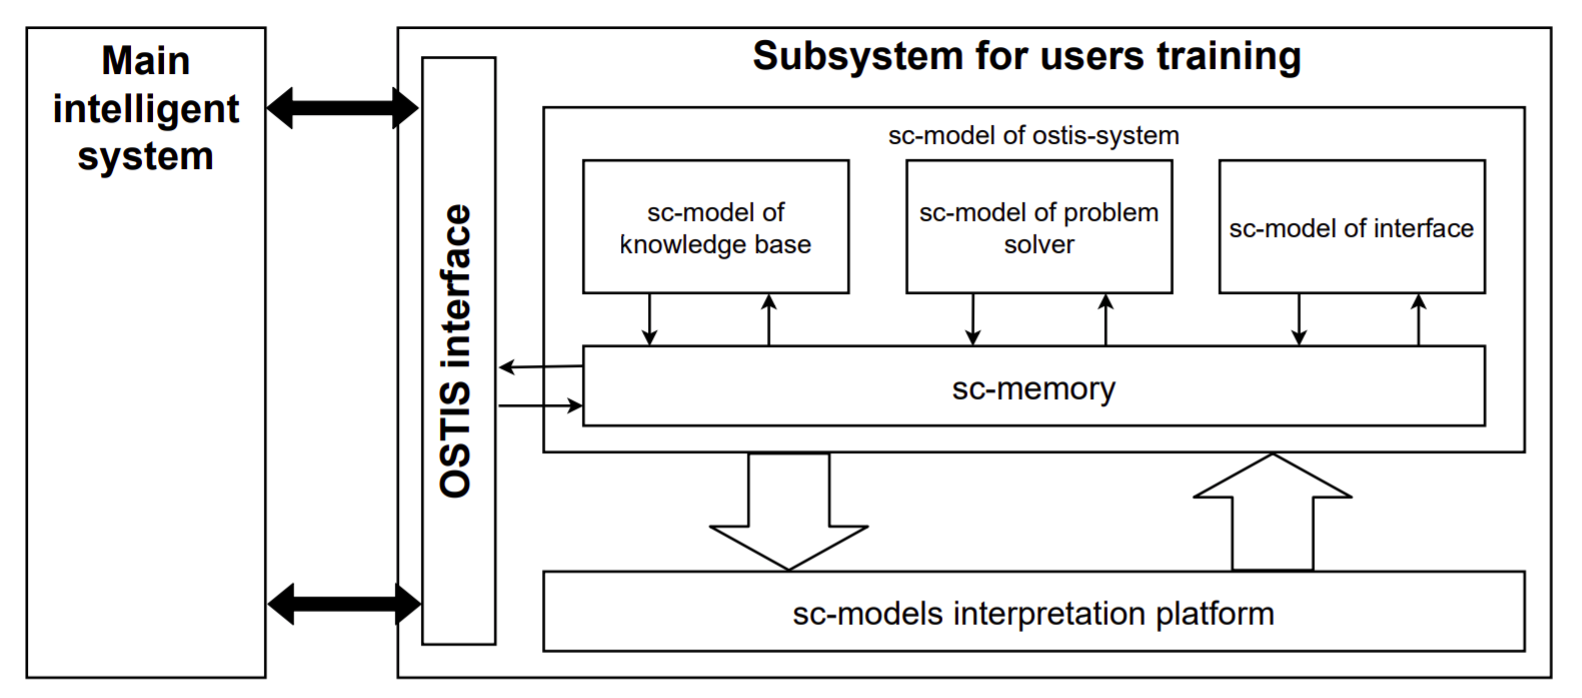
\includegraphics[width=0.8\linewidth]{images/part7/chapter_learning_systems/system_arch.png}
				%\caption{Пример рисунка в SCg-коде}
				\label{fig:system_arch}
			\end{figure}
		}
		\scnnote{В случае, если рассматриваемая интеллектуальная система является \textit{ostis-системой}, ее интеграция с подсистемой обучения пользователей интеллектуальных систем осуществляется более глубоко. Компоненты \textit{подсистемы обучения пользователей интеллектуальных систем} просто дополняют уже существующие в основной ostis-системе компоненты, что позволяет максимально снизить затраты на интеграцию \textit{подсистемы обучения пользователей интеллектуальных систем} и основной \textit{ostis-системы}.}
		\begin{scnindent}
			\scnrelfrom{иллюстрация}{
				\begin{figure}[H]
					\raggedleft
					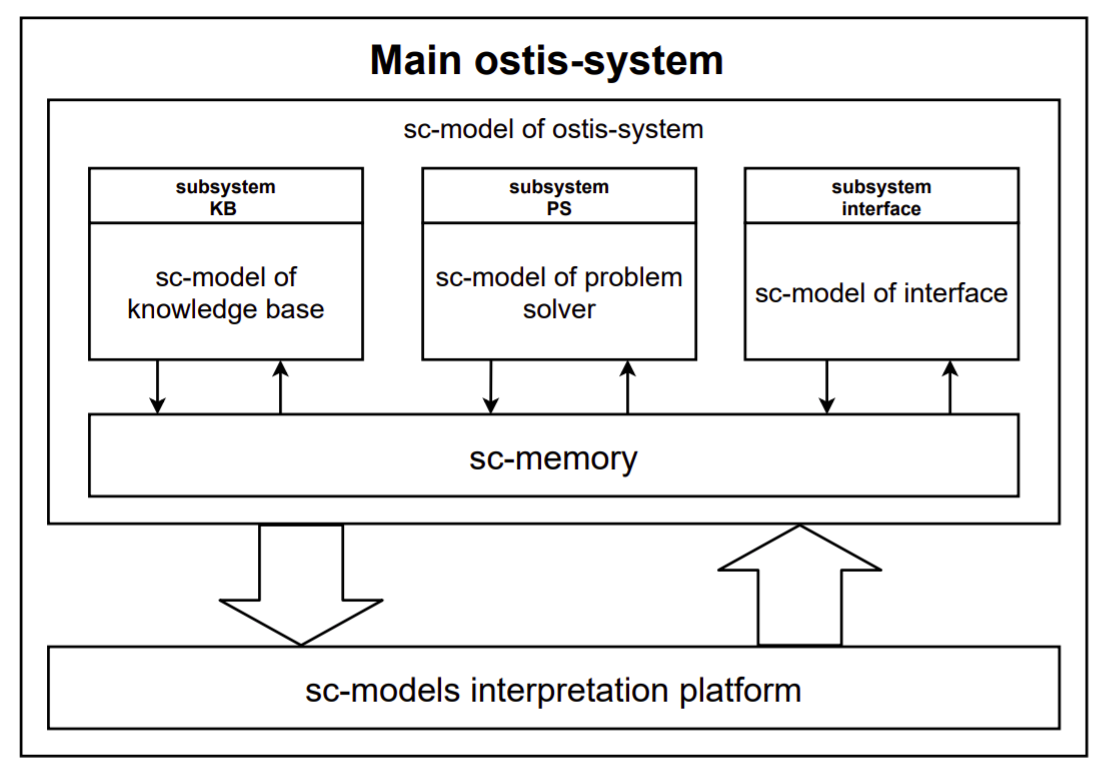
\includegraphics[width=0.8\linewidth]{images/part7/chapter_learning_systems/subsystem_arch.png}
					%\caption{Пример рисунка в SCg-коде}
					\label{fig:subsystem_arch.png}
				\end{figure}
			}
		\end{scnindent}
	\end{scnindent} 
\end{SCn}

\begin{SCn}
	\scnheader{интеллектуальная обучающая система}
	\scntext{часто используемый sc-идентификатор}{и.о.с.}
	\scnsubset{интеллектуальная система}
	\scnnote{Такого рода системы по сравнению с традиционными системами электронного обучения (например, электронными учебниками) предоставляют обладают рядом существенных преимуществ.}
	\scnsubset{интеллектуальная справочная система}
	\begin{scnindent}
		\scnexplanation{Каждая \textit{интеллектуальная обучающая система} в качестве простейшего средства изучения учебного материала предполагает наличие средств навигации по этому материалу и средств задания по нему различных вопросов. Системы, обладающие только таким ограниченным набором возможностей, названы \textit{интеллектуальными справочными системами}. Таким образом, можно сказать, что \textit{интеллектуальная обучающая система} обязательно реализует в себе функции \textit{интеллектуальной справочной системы}.}
	\end{scnindent} 
	\scnsuperset{интеллектуальная обучающая ostis-система}
	\begin{scnindent}
		\scnidtf{интеллектуальная обучающая система, построенная на основе Технологии OSTIS}
	\end{scnindent} 
\end{SCn}

\vspace{-\baselineskip}

Рассмотрим \textit{Преимущества интеллектуальных обучающих ostis-систем} в целом, а также их баз знаний, решателей задач и пользовательских интерфейсов.

\begin{SCn}
	\scnheader{интеллектуальная обучающая ostis-система}
	\begin{scnrelfromlistcustom}{обобщенная часть}
		\scnitemcustom{\textit{база знаний интеллектуальной обучающей ostis-системы}}
		\begin{scnindent}
		\begin{scnrelfromset}{преимущества}
			\scnfileitem{\textit{SC-код} позволяет представлять знания любого рода, в том числе конкретные факты, логические утверждения (аксиомы, теоремы, определения), текстовые и мультимедийные иллюстрации и комментарии, примеры конкретных задач с решениями, в том числе доказательства и так далее.}
			\scnfileitem{Пользователю становятся доступны достаточно полные сведения об изучаемой предметной области, отражены все ее аспекты, благодаря явному помещению в \textit{базу знаний} всех предметных закономерностей и взаимосвязей понятий.}
			\scnfileitem{\textit{База знаний} системы рассматривается как иерархия предметных областей и соответствующих им онтологий, то есть позволяет произвести семантическую структуризацию предлагаемого учащемуся материала, что существенно облегчает процесс обучения за счет систематизации знаний на основе именно их семантики, а не каких-либо других сторонних факторов. Кроме этого, знания в базе могут делиться на логические разделы, каждый из которых соответствует какому-либо фрагменту излагаемого материала. \textit{база знаний} позволяет осуществлять свободную навигацию по любым ассоциативным связям, изучая таким образом материал в той последовательности, какая кажется более логичной для самого обучаемого. С другой стороны, такой подход позволяет указать рекомендуемую последовательность изучения материала. При необходимости структура предметных областей может быть легко перестроена.}
			\scnfileitem{Пользователю в явном виде представляется семантическая структура изучаемого учебного материала и изучаемой предметной области. При этом обеспечивается наглядная визуализация любого уровня указанной семантической структуры.}
			\scnfileitem{Знания из различных областей представляются в схожем, подобном виде, что позволяет говорить не о семействе не связанных между собой обучающих систем по различным предметным областям, а о глобальном смысловом пространстве, объединяющем в себе знания всего семейства разрабатываемых систем. В свою очередь, наличие такого смыслового пространства обеспечивает ряд дополнительных возможностей:
			\begin{scnitemize}
				\item каждая система при необходимости может использовать знания, относящиеся к другим системам, что позволяется задавать не только вопросы, касающиеся конкретной предметной области, но и вопросы, носящие междисциплинарный характер;
				\item в рамках глобального смыслового пространства можно выделить часть знаний, которые имеют отношение ко многим системам из всего комплекса, например базовые знания из области математики, логики и так далее. Концепция глобального смыслового пространства позволяет записывать такие фрагменты знаний только в одной из систем, а затем использовать их во всех остальных, что существенно уменьшает количество дублирований, сокращает сроки разработки систем и снижает накладные расходы.
			\end{scnitemize}}
			\scnfileitem{Унифицированное представление знаний позволяет не ограничивать номенклатуру пользовательских запросов только специально выделенными для этого командами, а задавать произвольный запрос системе с использованием универсального языка отображения знаний, что делает перечень возможных запросов зависящим только от количества и разнообразия знаний, внесенных в базу знаний системы.}
		\end{scnrelfromset}
		\end{scnindent}
		
		\scnitemcustom{\textit{решатель задач интеллектуальной обучающей ostis-системы}}
		\begin{scnindent}
		\begin{scnrelfromset}{преимущества}
			\scnfileitem{Пользователю предоставляется возможность задавать системе любые вопросы и  задачи по изучаемой предметной области. Это достигается включением в и.о.с. решателя задач, способного решать задачи по их формулировкам, в том числе, введенным пользователем. При этом указанный решатель задач может находить путь решения задачи даже, если соответствующий способ решения (например, алгоритм) ему неизвестен.}
		\end{scnrelfromset}
		\end{scnindent} 
		
		\scnitemcustom{\textit{пользовательский интерфейс интеллектуальной обучающей ostis-системы}}
		\begin{scnindent}
		\begin{scnrelfromset}{преимущества}
			\scnfileitem{Унификация моделей пользовательских интерфейсов позволяет отображать знания различного рода в унифицированном виде независимо от предметной области, к которой эти знания относятся. Таким образом, все разрабатываемые системы будут обладать пользовательским интерфейсом, построенным по одним и тем же принципам, что позволит существенно сократить срок ознакомления учащегося со всем семейством систем. Данный факт не отрицает возможность и необходимость разработки отдельных компонентов интерфейса, ориентированных на конкретную предметную область, например, редактора геометрических чертежей, виртуальной лаборатории для проведения химических опытов и так далее.}
			\scnfileitem{и.о.с. имеет интеллектуальный пользовательский интерфейс с компьютерными (виртуальными) моделями различных объектов изучаемой предметной области, что позволяет системе "понимать"{} смысл (анализировать семантику) пользовательских действий по преобразованию этих объектов. Все это существенно повышает уровень интерактивной виртуальной лабораторной среды электронного учебника.}
			\scnfileitem{Каждый компонент пользовательского интерфейса также является отображением определенного элемента из базы знаний, что позволяет, во-первых, легко менять интерфейс системы даже во время ее работы, а, во-вторых, позволяет пользователю задавать системе вопросы не только касательно предметной области, которой посвящена данная система, но и касательно любого из компонентов интерфейса и других частей системы. Таким образом, пользователю достаточно научиться задавать системе несколько простейших вопросов, чтобы в дальнейшем изучить все тонкости работы системой уже в процессе общения с ней.}
			\scnfileitem{При общении с системой пользователю предоставляется свобода в выборе любого из множества синонимичных терминов (идентификаторов), зарегистрированных в \textit{базе знаний} системы. При этом указанные термины могут принадлежать различным естественным языкам.}
			\scnfileitem{Появляется принципиальная возможность реализации естественно-языкового интерфейса с пользователем (благодаря широким возможностям семантического анализа пользовательских сообщений и возможностям синтеза на семантическом уровне сообщений, адресуемых пользователям).}
			\scnfileitem{Достаточно легко осуществляется переориентация и.о.с. на обслуживание пользователей с другим естественным языком (так как основная часть базы знаний и.о.с., непосредственно описывающая семантику соответствующей предметной области, абсолютно не зависит от внешнего  языка, в том числе от естественного).}
		\end{scnrelfromset}
		\end{scnindent} 
	\end{scnrelfromlistcustom}
	
	\begin{scnrelfromset}{преимущества}
		\scnfileitem{Помимо возможности чтения текстов и иллюстративных материалов учебника предоставляется возможность навигации по семантическому пространству предметной области.}
		\scnfileitem{Пользователю предоставляется возможность под контролем системы тренироваться (приобретать практические навыки) в решении самых различных задач по изучаемой предметной области. При этом система
		\begin{scnitemize}
			\item осуществляет семантический анализ правильности решения задач как по свободно конструируемым ответам (результатам), так и по протоколам решения;
			\item локализует допущенные пользователем ошибки в решении задач, определяет их причину и выдает соответствующие рекомендации пользователю.
		\end{scnitemize}}
		\scnfileitem{Пользователю предоставляется полная свобода в выборе последовательности изучения учебного материала (маршрута навигации по учебному материалу). Тем не менее, система выдаёт соответствующие рекомендации.}
		\scnfileitem{Пользователю предоставляется полная свобода в выборе решаемых им задач (в сборнике задач и лабораторных работ), но соответствующие рекомендации выдаются \textit{интеллектуальной обучающей ostis-системой}. Эти рекомендации направлены на то, чтобы минимизировать число решаемых задач, обеспечивающих приобретение требуемых практических навыков.}
		\scnfileitem{Достаточно легко осуществляется интеграция нескольких самостоятельных и.о.с. по смежным дисциплинам в единый учебник, что, в частности, предоставляет возможность задавать вопросы и задачи на стыке этих дисциплин.}
		\scnfileitem{Пользователь и.о.с. работает под наблюдением и контролем интеллектуального персонального ассистента, который помогает пользователю быстро и эффективно освоить возможности системы. По сути это не что иное, как руководство пользователя и.о.с., оформленное как семантический электронный учебник.}
		\scnfileitem{При проектировании базы знаний и.о.с. появляется уникальная возможность проверять семантическую корректность формируемого информационного ресурса:
			\begin{scnitemize}
				\item корректность определений и утверждений;
				\item корректность использования различных понятий;
				\item корректность алгоритмов;
				\item корректность доказательств теорем;
				\item и так далее.
		\end{scnitemize}}
	\end{scnrelfromset}
	\begin{scnindent}
		\scnnote{Часть из перечисленных возможностей (а в предельном случае и все их них) могут быть реализованы в рамках \textit{подсистемы обучения пользователей интеллектуальных систем}.}
	\end{scnindent} 
\end{SCn}